%%%%%%%%%%%%%%%%%%%%%%%%%%%%%%%%%%%%%%%%%%%%%%%%%%%%%%
\documentclass[11pt]{article}
%%%%%%%%%%%%%%%%%%%%%%%%%%%%%%%%%%%%%%%%%%%%%%%%%%%%%%

\usepackage{amsmath}
\usepackage{amsthm}
\usepackage{amssymb}
\usepackage{latexsym}
\usepackage{graphicx}
\usepackage{color}
\usepackage{verbatim}
\usepackage{float}
\usepackage{multicol}
\usepackage{xcolor}
\usepackage{listings}
\usepackage{tikz}
\usetikzlibrary{arrows.meta, positioning, calc}
\usetikzlibrary{decorations.pathmorphing}
\usepackage{tcolorbox}
\tcbuselibrary{breakable}

\newtcolorbox{solutionbox}{
  breakable,
  colback=blue!5!white,
  colframe=blue!50!black,
  title=Solution,
  sharp corners,
  boxrule=0.8pt
}

\newtcolorbox{hintbox}{
  breakable,
  colback=gray!10!white,
  colframe=gray!50!black,
  title=Hint,
  sharp corners,
  boxrule=0.5pt
}

% Unnumbered theorem
\newtheorem*{thm*}{Theorem}


\lstdefinelanguage{R}{
      keywords={if,else,while,for,in,next,break,function,TRUE,FALSE,NULL,Inf,NA,NaN,switch,repeat,return,require,library},
      keywordstyle=\color{blue}\bfseries,
      identifierstyle=\color{black},
      comment=[l]{\#},
      commentstyle=\color{gray}\ttfamily,
      string=[b]{"},
      stringstyle=\color{red}\ttfamily,
      morecomment=[l]{//},
      morestring=[b]{'},
      sensitive=true,
      morekeywords={print,summary,plot,lm,glm,data,frame,read.csv,write.csv,factor,levels,names,colnames,rownames,
      head,tail,str,dim,length,class,typeof,mode,is.na,is.null,is.finite,is.infinite,is.nan,as.numeric,as.character,
      as.factor,as.Date,as.POSIXct,as.matrix,as.data.frame,rbind,cbind,merge,subset,aggregate,tapply,apply,lapply,sapply,
      mapply,vapply,replicate,seq,rep,c,list,matrix,array,data.frame,table,hist,boxplot,barplot,pie,curve,lines,points,text,
      abline,legend,par,mtext,title,xlab,ylab,xlim,ylim,main,sub,col,pch,cex,lty,lwd,type,bg,fg,args,options,warnings,errors,
      message,stop,warning,error,try,tryCatch,withCallingHandlers,on.exit,debug,browser,trace,recover,options,getOption,setOption},
    }


\setlength{\textheight}{9in}
\setlength{\textwidth}{6in}
\addtolength{\topmargin}{-2cm}
\addtolength{\oddsidemargin}{-1cm}
\parindent=0in


\def\classnum{3810}
\def\classtitle{Probability}
\def\classtitleshort{Probability}
\def\classsec{001}
\def\classterm{Fall 2025}
\def\instructor{Robert Rostermundt}
%\def\hmwknum{\#2}


%%%%%%%%%%%%%%%%%%%%%%%%%%%%%%%%%%%%%%%%%%%%%%%%%%%%%%%%%
%%%%%%%%%%%%%%%%%%%%%%%%%  Colors  %%%%%%%%%%%%%%%%%%%%%%
%%%%%%%%%%%%%%%%%%%%%%%%%%%%%%%%%%%%%%%%%%%%%%%%%%%%%%%%%

\definecolor{Green}{rgb}{0,.5,0}
%use for definitions
\definecolor{Red}{rgb}{.8,.2,0}
%use for emphasis
\definecolor{Yellow}{rgb}{.6,.6,.1}
%use for part titles
\definecolor{Cyan}{rgb}{.2,.6,.7}
%use for comments
\definecolor{Purple}{rgb}{.4,0,1}
%use for examples
\definecolor{deepred}{rgb}{.53,.29,.24}
%use for important points
\definecolor{Black}{rgb}{0,0,0}
%use for washout
\definecolor{Grey}{rgb}{.45,.45,.45}
% use for theorems
\newcommand{\tred}[1]{\textcolor{Red}{#1}}
\newcommand{\tgreen}[1]{\textcolor{Green}{#1}}
\newcommand{\tcyan}[1]{\textcolor{Cyan}{#1}}
\newcommand{\tyellow}[1]{\textcolor{Yellow}{#1}}
\newcommand{\tpurple}[1]{\textcolor{Purple}{#1}}
\newcommand{\tblack}[1]{\textcolor{Black}{#1}}
\newcommand{\tgrey}[1]{\textcolor{Grey}{#1}}
\newcommand{\tdeepred}[1]{\textcolor{deepred}{#1}}
\newcommand{\ttt}[1]{\texttt{#1}}

%%%%%%%%%%%%%%%%%%%%%%%%%%%%%%%%%%%%%%%%%%%%%%%%%%%%%%%%%
%%%%%%%%%%%%%%%%%%%%%%%%%  Theorem Environments  %%%%%%%%
%%%%%%%%%%%%%%%%%%%%%%%%%%%%%%%%%%%%%%%%%%%%%%%%%%%%%%%%%

\theoremstyle{plain}
\newtheorem{thm}{Theorem}
\newtheorem{axiom}{Axiom}
\newtheorem{cor}{Corollary}
\newtheorem{lemma}{Lemma}
\newtheorem{prop}{Proposition}
\newtheorem{ques}{Question}
\theoremstyle{definition}
\newtheorem{defn}{Definition}
\theoremstyle{remark}
\newtheorem{remark}{Remark}
\theoremstyle{definition}
\newtheorem{ex}{Example}
\numberwithin{equation}{section}
\newtheorem{prob}{Problem}
\numberwithin{equation}{section}


%%%%%%%%%%%%%%%%%%%%%%%%%%%%%%%%%%%%%%%%%%%%%%%%%%%%%%%%%
%%%%%%%%%%%%%%%%%%%%%%%%%  Math    %%%%%%%%%%%%%%%%%%%%%%
%%%%%%%%%%%%%%%%%%%%%%%%%%%%%%%%%%%%%%%%%%%%%%%%%%%%%%%%%


\newcommand{\abs}[1]{\left\lvert{#1}\right\rvert}
\newcommand{\card}[1]{\lvert{#1}\rvert}
\newcommand{\union}{\cup}
\newcommand{\Union}{\bigcup}
\newcommand{\inter}{\cap}
\newcommand{\Inter}{\bigcap}
%\newcommand{\hint}[1]{\medskip\newline\emph{Hint: #1}}
%\newcommand{\note}[1]{\medskip\newline\emph{Note: #1}}
\newcommand{\points}[1]{[#1 points]}
\newcommand{\totalpoints}[1]{[#1 points total]}
\newcommand{\ds}{\displaystyle}
\newcommand{\ben}{\begin{enumerate}}
\newcommand{\een}{\end{enumerate}}
\newcommand{\bi}{\begin{itemize}}
\newcommand{\ei}{\end{itemize}}
\newcommand{\beq}{\begin{eqnarray*}}
\newcommand{\eeq}{\end{eqnarray*}}
\newcommand{\bieq}{\begin{IEEEeqnarray}{rCl}}
\newcommand{\bieqx}{\begin{IEEEeqnarray}{+rCl+x*}}
\newcommand{\eieq}{\end{IEEEeqnarray}}
\newcommand{\nn}{\nonumber}
%\renewcommand{\i}{\item}
\newcommand{\bpm}{\begin{pmatrix}}
\newcommand{\epm}{\end{pmatrix}}
\newcommand{\sol}{\indent{\bf\emph{Solution:}}}
\newcommand{\ssol}{\indent{\\[2mm]\bf\emph{Solution:}}\;}
\newcommand{\hint}{\indent{\bf\emph{Hint}:}\;}
\newcommand{\note}{\indent{\bf\emph{Note}:}\;}
\newcommand{\vsk}{\vskip 2mm}
%%%%%%%%%%%%%%%%%%%%%%%%% Calculus %%%%%%%%%%%%%%%%%%%%%%%%%%%%
\newcommand{\dd}[2]{\ds\frac{d}{d{#1}}\left[{#2}\right]}
\newcommand{\der}[2]{\ds\frac{d{#1}}{d{#2}}}
\newcommand{\lmt}[3]{\ds\lim_{{#1}\to{#2}}{#3}}
\renewcommand{\iint}[2]{\ds\int{#1}\,d{#2}}
\newcommand{\dint}[4]{\ds\int^{#4}_{#3}{#1}\,d{#2}}
\renewcommand{\Delta}{\triangle}
%%%%%%%%%%%%%%%%%%%%%%%%% Number Sets %%%%%%%%%%%%%%%%%%%%%%%%%%
\newcommand{\N}{\mathbb{N}}
\newcommand{\Z}{\mathbb{Z}}
\newcommand{\Q}{\mathbb{Q}}
\newcommand{\R}{\mathbb{R}}
\newcommand{\C}{\mathbb{C}}
\newcommand{\F}{\mathcal{F}}
\renewcommand{\P}{\mathbb{P}}
\newcommand{\E}{\mathcal{E}}
\renewcommand{\o}{\omega}
\renewcommand{\O}{\Omega}
%%%%%%%%%%%%%%%%%%%%%%%%% Vectors %%%%%%%%%%%%%%%%%%%%%%%%%%%%%
\newcommand{\x}{\bar{x}}
\renewcommand{\v}{\bar{v}}
\newcommand{\y}{\bar{y}}
\newcommand{\z}{\bar{z}}
\newcommand{\w}{\bar{w}}
\renewcommand{\u}{\bar{u}}
\renewcommand{\b}{\bar{b}}
\newcommand{\e}{\bar{e}}
\renewcommand{\a}{\vec{a}}
\renewcommand{\r}{\vec{r}}
\newcommand{\vv}{\vec{v}}
\newcommand{\vecPQ}[2]{\overrightarrow{#1}{#2}}
\newcommand{\vecV}[1]{\overrightarrow{#1}}
\newcommand{\la}{\langle}
\newcommand{\ra}{\rangle}
%%%%%%%%%%%%%%%%%%%%%%%%%%% Vector Spaces %%%%%%%%%%%%%%%%%%%%
\newcommand{\rn}{\ensuremath{\mathbb{R}^n}}
\renewcommand{\rm}{\ensuremath{\mathbb{R}^m}}
\newcommand{\re}{\mathbb{R}}
\newcommand{\Pn}{\mathbb{P}_n}
\newcommand{\B}{\mathcal{B}}
%%%%%%%%%%%%%%%%%%%%%%%%%%% Graphics %%%%%%%%%%%%%%%%%%%%%%%%
\newcommand{\cg}[2]{\begin{center}
\includegraphics[scale={#1}]{{#2}}
\end{center}}
\makeatletter
\def\imod#1{\allowbreak\mkern10mu({\operator@font mod}\,\,#1)}
\makeatother

%%%%%%%%%%%%%%%%%%%%%%%%%%%%%%%%%%%%%%%%%%%%%%%%%%%%%%%%%%%%%%%%%%%%%%%%%%%%%%%%%%%%%%%%%%%%%%
%%%%%%%%%%%%%%%%%%%%%%%%%%%%%% Defined Fonts %%%%%%%%%%%%%%%%%%%%%%%%%%%%%%%%%%%%%%%%%%%%%%%%%
%%%%%%%%%%%%%%%%%%%%%%%%%%%%%%%%%%%%%%%%%%%%%%%%%%%%%%%%%%%%%%%%%%%%%%%%%%%%%%%%%%%%%%%%%%%%%%

\font\minihelv=phvr at 6pt
\font\helv=phvr at 10pt
\font\medhelv=phvr at 16pt
\font\bighelv=phvr at 20pt
\font\hugehelv=phvr at 36pt
\font\mybigfont=phvr at 16pt
\font\mymediumfont=phvr at 14pt
\font\mediumhelv=phvr at 14pt
\font\mybfit=ptmbi at 12pt


%%%%%%%%%%%%%%%%%%%%%%%%%%%%%%%%%%%%%%%%%%%%%%%%%%%%%%%%%%%%%%%%%%%%%%%%%%%%%%%%%%%%%%%%%%%%%%%
%%%%%%%%%%%%%%%%%%%%%%%%%%%%%% Other Commands %%%%%%%%%%%%%%%%%%%%%%%%%%%%%%%%%%%%%%%%%%%%%%%%%
%%%%%%%%%%%%%%%%%%%%%%%%%%%%%%%%%%%%%%%%%%%%%%%%%%%%%%%%%%%%%%%%%%%%%%%%%%%%%%%%%%%%%%%%%%%%%%%
%\setlength\fboxrule{.5pt}
%\newcommand{\latexpicborder}[3]{
%\setlength\fboxsep{30pt}
%\begin{figure}[hb]
%\begin{center}
%\fbox{
%\input{#1}
%}
%\caption{#2}
%\label{#3}
%\end{center}
%\end{figure}
%\setlength\fboxsep{0pt}
%}
%
%\newcommand{\latexpic}[2]{
%\begin{figure}[hb]
%\begin{center}
%\input{#1}
%\vspace*{8mm}
%\caption{#2}
%\end{center}
%\end{figure}
%}

%\begin{minipage}[b]{0.6\linewidth}
%......
%\end{minipage}
%\hspace{0.5cm}
%\begin{minipage}[t]{0.4\linewidth}
%\centering
%\includegraphics[scale=.5]{m1401_ex3_g4.eps}
%\end{minipage}
%\end{figure}


%%%%%%%%%%%%%%%%%%%%%%%%%%%%%%%%%%%%%%%%%%%%%%%%%%%%%%%%%%%%%%%%%%%%%%%%%%%%%%%%%%%%%%%%%%%%%%
%%%%%%%%%%%%%%%%%%%%%%%%%%% IEEEeqnarray Notes %%%%%%%%%%%%%%%%%%%%%%%%%%%%%%%%%%%%%%%%%%%%%%%
%%%%%%%%%%%%%%%%%%%%%%%%%%%%%%%%%%%%%%%%%%%%%%%%%%%%%%%%%%%%%%%%%%%%%%%%%%%%%%%%%%%%%%%%%%%%%%


%Any number of columns can be specified with IEEEeqnarray: {c} will give only one
%column with all entries centered, or {rCll} would add a fourth, left-justified
%column to use for comments. Moreover, beside l, c, r, L, C, R for math mode
%entries there are also s, t, u for left, centered, and right text mode entries.
%Additional space can be added with . and / and ? in increasing order.
%
%
%\begin{proof}
%This is a proof that ends
%with an equation array:
%\begin{IEEEeqnarray*}{+rCl+x*}
%a & = & b + c \\
%& = & d + e. & \qedhere
%\end{IEEEeqnarray*}
%\end{proof}
%Note that the + in {+rCl+x*} denotes stretchable spaces, one on the left
%of the equations (which, if not specified, will be done automatically by
%IEEEeqnarray!) and one on the right of the equations. But now on the right,
%after the stretching column, we add an empty column x. This column will be
%only needed on the last line when we will put the \qedhere command there.
%Finally, we specify a *. This is a null-space that prevents IEEEeqnarray to
%add another unwanted +-space!


% The following environments enable custom numbering of theorems so that the numbers agree % with the numbering in the textbook being used. 
%
%  Usage examples:
%\begin{customthm}{2.2}\label{eight}
%Every theorem must be numbered by hand.
%\end{customthm}
%
%Here is a reference to theorem~\ref{eight}.
%
%\begin{customthm}{2.3}[Parenthetical comment]\label{nine}
%Statement
%\end{customthm}
%
%Here is a reference to theorem~\ref{nine}


\newtheorem{innercustomthm}{Theorem}
\newenvironment{customthm}[1]
  {\renewcommand\theinnercustomthm{#1}\innercustomthm}
  {\endinnercustomthm}
  
  \newtheorem{innercustomprop}{Proposition}
\newenvironment{customprop}[1]
  {\renewcommand\theinnercustomprop{#1}\innercustomprop}
  {\endinnercustomprop}
  
    \newtheorem{innercustomlem}{Lemma}
\newenvironment{customlem}[1]
  {\renewcommand\theinnercustomlem{#1}\innercustomlem}
  {\endinnercustomlem}
  
    \newtheorem{innercustomconj}{Conjecture}
\newenvironment{customconj}[1]
  {\renewcommand\theinnercustomconj{#1}\innercustomconj}
  {\endinnercustomconj}
  
    \newtheorem{innercustomclaim}{Claim}
\newenvironment{customclaim}[1]
  {\renewcommand\theinnercustomclaim{#1}\innercustomclaim}
  {\endinnercustomclaim}
  
    \newtheorem{innercustomcor}{Corollary}
\newenvironment{customcor}[1]
  {\renewcommand\theinnercustomcor{#1}\innercustomcor}
  {\endinnercustomcor}
  
    \newtheorem{innercustomdef}{Definition}
\newenvironment{customdef}[1]
  {\renewcommand\theinnercustomdef{#1}\innercustomdef}
  {\endinnercustomdef}
  
    \newtheorem{innercustomex}{Example}
\newenvironment{customex}[1]
  {\renewcommand\theinnercustomex{#1}\innercustomex}
  {\endinnercustomex}
  
    \newtheorem{innercustomass}{Assumption}
\newenvironment{customass}[1]
  {\renewcommand\theinnercustomass{#1}\innercustomass}
  {\endinnercustomass}
  
      \newtheorem{innercustomax}{Axiom}
\newenvironment{customax}[1]
  {\renewcommand\theinnercustomax{#1}\innercustomax}
  {\endinnercustomax}
  

\vfuzz2pt % Don't report over-full v-boxes if over-edge is small
\hfuzz2pt % Don't report over-full h-boxes if over-edge is small

\renewcommand{\ni}{\noindent}


%%%%%%%%%%%%%%%%%%%%%%%%%%%%%%%%%%%%%%%%%%%%%%%%%%%%%%
%%%%%%%%%%%%%%%%%%%%%%%%%%%%%%%%%%%%%%%%%%%%%%%%%%%%%%

\pagestyle{myheadings}

%%%%%%%%%%%%%%%%%%%%%%%%%%%%%%%%%%%%%%%%%%%%%%%%%%%%%%

%%%%%%%%%%%%%%%%%%%%%%%%%%%%%%%%%%%%%%%%%%%%%%%%%%%%%%
%%%%%%%%%%%%%%%%%%%%%%%%%   Document Body   %%%%%%%%%%
%%%%%%%%%%%%%%%%%%%%%%%%%%%%%%%%%%%%%%%%%%%%%%%%%%%%%%

%\def\classnum{3810}
%\def\classtitle{Probability}
%\def\classtitleshort{Probability}
%\def\classsec{001}
%\def\classterm{Fall 2025}
%\def\instructor{Robert Rostermundt}
\def\printsol{0}


	\title{\vspace{-1in}Math\classnum\;-\;\classtitle\\
	Section\;\classsec\;-\;\classterm\\
	Notes: Geometric Random Variables}
	\author{University of Colorado Denver / College of Liberal Arts 	and Sciences}
	\date{Department of Mathematics - \instructor}

	\markright{Math\classnum\;-\;\classtitleshort, UCD, \classterm, \instructor}



%%%%%%%%%%%%%%%%%%%%%%%%%%%%%%%%%%%%%%%%%%%%%%%%%%%%%%
\begin{document}\maketitle\thispagestyle{empty}
%%%%%%%%%%%%%%%%%%%%%%%%%%%%%%%%%%%%%%%%%%%%%%%%%%%%%%



%%%%%%%%%%%%%%%%%%%%%%%%%%%%%%%%%%%%%%%%%%%%%%%%%%%%%%%%%%%%%%%%%%%%%%%%%%%%%%%%%%%%%%%%%%%%%%%%%%%%%%
\vspace*{2mm}
\hrule
\vskip 8mm


%%%%%%%%%%%%%%%%%%%%%%%%%%%%%%%%%%%%%%%%%%%%%%%%%%%%%%%%%%%%%%%%%%%%%%%%%
%%%%%%%%%%%%%%%%%%%%%%%%%%%%%%%%%%%%%%%%%%%%%%%%%%%%%%%%%%%%%%%%%%%%%%%%%





%--------------------------------
% Optional diagram
%--------------------------------
%\begin{figure}[h!]
%\centering
%\begin{tikzpicture}[x=0.9cm,y=1cm]
%
%% ------------------------
%% PARAMETERS
%% ------------------------
%\def\K{4}      % number of failures after first trial
%\def\END{7}    % rightmost underline index (after removing last two)
%
%% ------------------------
%% DERIVED INDICES (PRECOMPUTED)
%% ------------------------
%\pgfmathtruncatemacro{\UPTO}{\K+1}        % last underline before dots
%\pgfmathtruncatemacro{\KD}{\K+2}          % dots anchor
%
%% ------------------------
%% Top row: X
%% ------------------------
%\node at (-1,0) {$X:$};
%
%% Underlines up to dots
%\foreach \i in {0,...,\UPTO} {
%  \draw (\i,0) -- (\i+0.7,0);
%}
%
%% Dots (shifted slightly right)
%\node[xshift=0.35cm] at (\KD,0) {\Large $\dots$};
%
%% ------------------------
%% Bottom row: X - 1
%% ------------------------
%\node at (-1,-1) {$X-1:$};
%
%% Underlines up to dots (start under 2nd slot)
%\foreach \i in {1,...,\UPTO} {
%  \draw (\i,-1) -- (\i+0.7,-1);
%}
%
%% Dots (shifted slightly right)
%\node[xshift=0.35cm] at (\KD,-1) {\Large $\dots$};
%
%% ------------------------
%% Conditioning bar
%% ------------------------
%\draw (0.85,-0.35) -- (0.85,0.35);
%
%% Failures
%\node at (0.35,0.45) {\small F};
%\foreach \i in {1,...,\K} {
%  \node at (\i+0.35,0.45) {\small F};
%}
%
%% Failures in shifted process
%\foreach \i in {1,...,\K} {
%  \node at (\i+0.35,-0.55) {\small F};
%}
%
%% ------------------------
%% Probability explanation
%% ------------------------
%\node at (3.8,-2.2)
%{\small $\Pr(X > 4) = \Pr(X > 4+1 \mid X > 1)$};
%
%\end{tikzpicture}
%\caption{Memoryless property of the geometric distribution.}
%\end{figure}




%%%%%%%%%%%%%%%%%%%%%%%%%%%%%%%%%%%%%%%%%%%%%%%%%%%%%%%%%%%%%%%%%%%%%%%%%%%%%%%%%%%%%%%%%%%%%%%%%%%%%%
\section*{The Problem:}
%%%%%%%%%%%%%%%%%%%%%%%%%%%%%%%%%%%%%%%%%%%%%%%%%%%%%%%%%%%%%%%%%%%%%%%%%%%%%%%%%%%%%%%%%%%%%%%%%%%%%%


\noindent Consider a sequence of independent Bernoulli trials (such as tossing a coin) where we are waiting for the first ``success." If we let $X$ be the number of trials until we see the first success, then $X$ is a geometric random variable: $X\sim Geom(p)$. We would like to know the expected number of trials (on average) until we see the first success. We need to evaluate
\[E[X]=\ds\sum^{\infty}_{k=1}x\cdot p_{_X}(k)=\ds\sum^{\infty}_{k=1}k\cdot(1-p)^{k-1}p.\]


%%%%%%%%%%%%%%%%%%%%%%%%%%%%%%%%%%%%%%%%%%%%%%%%%%%%%%%%%%%%%%%%%%%%%%%%%%%%%%%%%%%%%%%%%%%%%%%%%%%%%%
\section*{Theoretical Tools:}
%%%%%%%%%%%%%%%%%%%%%%%%%%%%%%%%%%%%%%%%%%%%%%%%%%%%%%%%%%%%%%%%%%%%%%%%%%%%%%%%%%%%%%%%%%%%%%%%%%%%%%

\begin{itemize}
	\item Memoryless Property: If $X\sim Geom(p)$, then $\P(X>s+t\,|\,X>t)=\P(X>s)$.
	\item Law of Total Expectation: Suppose $(\O,\F,\P)$ is a probability space and there are events $A_1,A_2,\dots,A_n\in\F$ that partition the sample space. Then we have
\[E[X]=\P(A_1)\cdot\mathbb{E}[X\,|\,A_1]+\cdots+\P(A_n)\cdot\mathbb{E}[X\,|\,A_n].\]	
	\item Geometric Sums: If $|r|<1$ we have $\sum^{\infty}_{k=0}r^k=\frac{1}{1-r}$. Moreover, we can differentiate a geometric sum term-by-term. This gives us
\[\sum^{\infty}_{k=1}kr^{k-1}=\frac{d}{dr}\left[\sum^{\infty}_{k=0}r^k\right]=\frac{d}{dr}\left[\frac{1}{1-r}\right]=\ds\frac{1}{(1-r)^2}.\]
\end{itemize}

%%%%%%%%%%%%%%%%%%%%%%%%%%%%%%%%%%%%%%%%%%%%%%%%%%%%%%%%%%%%%%%%%%%%%%%%%%%%%%%%%%%%%%%%%%%%%%%%%%%%%%
\section*{Calculations:}
%%%%%%%%%%%%%%%%%%%%%%%%%%%%%%%%%%%%%%%%%%%%%%%%%%%%%%%%%%%%%%%%%%%%%%%%%%%%%%%%%%%%%%%%%%%%%%%%%%%%%%

\noindent 

Suppose $X \sim \text{Geom}(p)$, so that $\P(X=k)=(1-p)^{k-1}p, \quad k=1,2,3,\dots$. 
\beq
\mathbb{E}[X]&=&\sum_{k=1}^{\infty}k\cdot\P(X=k)\\ 
&=&\sum_{k=1}^{\infty} k(1-p)^{k-1}p\\
&=&p\sum_{k=1}^{\infty} k (1-p)^{k-1} \\
\eeq
Let $r= 1-p$. Then $\sum_{k=1}^{\infty} k r^{k-1}=\sum_{k=0}^{\infty} k r^{k-1}$ is needed. Recall
\[\sum_{k=0}^{\infty} r^k = \frac{1}{1-r} \implies \sum_{k=0}^{\infty} k r^{k-1}=\frac{d}{dr}\left[\sum_{k=0}^{\infty}r^k\right]=\frac{d}{dr}\left[\ds\frac{1}{1-r}\right]=\frac{1}{(1-r)^2}.\]
So we have
\[\sum_{k=1}^{\infty} k r^{k-1}=\frac{1}{(1-r)^2}=\frac{1}{p^2}\Longrightarrow\mathbb{E}[X]=p\cdot \frac{1}{p^2}=\frac{1}{p}.\]
\vskip 5mm

\noindent \textbf{Intuition for } $\mathbb{E}[X] = 1/p$: 
$X$ counts the number of trials until the first success. On average, 
it takes $1/p$ trials to see a success:

\begin{itemize}
\item $p=1/2$: expect $2$ trials (makes sense for a fair coin). 
\item $p=0.01$: expect $100$ trials (success is unlikely and rare, so wait longer). 
\item $p=1$: expect $1$ trial (always succeed immediately). 
\end{itemize}

How about the variance?


\[X\sim \text{Geom}(p), \quad \P(X=k)=p(1-p)^{k-1}, \quad k=1,2,3,\dots\]
\vskip 5mm
Now let $q=1-p$. Then we have
\begin{align*}
\mathbb{E}[X^2] &= \mathbb{E}[X(X-1)] + \mathbb{E}[X] 
 =p\sum_{k=0}^{\infty} k(k-1) q^{k-1} + \frac{1}{p} \\[1mm]
&=p\cdot\frac{d^2}{dq^2}\left[\sum_{k=0}^{\infty}q^k\right] + \frac{1}{p} 
 =p\cdot\frac{d^2}{dq^2}\left[\frac{1}{1-q}\right] + \frac{1}{p} \\[1mm]
&=p\cdot \frac{2}{(1-q)^3} + \frac{1}{p} 
 =p\cdot \frac{2}{p^3} + \frac{1}{p} 
 = \frac{2-p}{p^2}.
\end{align*}
From this we conclude that
\[\mathrm{Var}(X)=E\left[X^2\right]-\left(E[X]\right)^2=\frac{2-p}{p^2}-\ds\frac{1}{p^2}=\ds\frac{1-p}{p^2}.\]
\vskip 5mm

\noindent \textbf{Intuition for } $\mathrm{Var}(X) = \frac{1-p}{p^2}$:
\begin{itemize}
\item If $p$ is large (success likely), waiting times are tightly clustered near $1$, so variance is small.
\item If $p$ is small (success rare), waiting times can vary a lot, so variance is large.
%\item The factor $1/p^2$ scales with the square of the average waiting time, and the factor $1-p$ accounts for the "failure randomness" in each trial.
\end{itemize}

\vskip 1cm

\paragraph*{Using the Memoryless Property:}

A more elegant approach uses the memoryless property. We assume $X\sim\text{Geom}(p)$ (number of trials until first success). We see that the events $X=1$ and $X>1$ partition the sample space and we use the law of total expectation.
\vskip 5mm
\begin{figure}[h!]
\centering
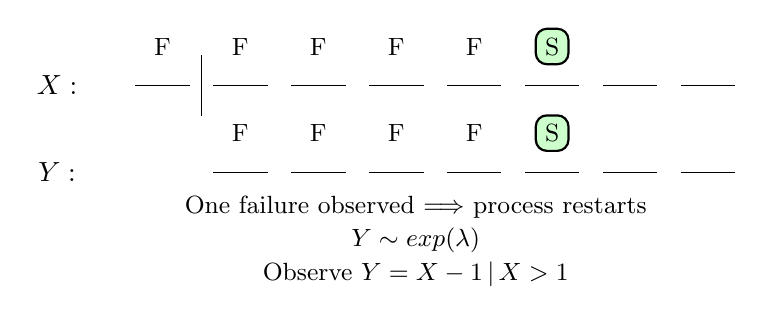
\begin{tikzpicture}[scale=1.1,x=0.9cm,y=1cm]

% PARAMETERS
\def\K{6}      % x-position index of success
\def\END{7}    % right endpoint (top row)

% ------------------------
% Top row: X
% ------------------------
\node at (-1,0) {$X:$};

% Underlined Bernoulli trials (top row)
\foreach \i in {0,...,\END} {
  \draw (\i,0) -- (\i+0.7,0);
}

% Failure labels before success
\foreach \i in {0,...,\numexpr\K-2} {
  \node at (\i+0.35,0.45) {\small F};
}

% Success at trial k
\node[draw, thick, rounded corners, fill=green!20]
  at (\K-0.65,0.45) {\small S};

% Conditioning bar after first trial
\draw (0.85,-0.35) -- (0.85,0.35);

% ------------------------
% Bottom row: X - 1
% ------------------------
\node at (-1,-1) {$Y:$};

% Underlined Bernoulli trials (start under 2nd slot of X)
\foreach \i in {1,...,\END} {
  \draw (\i,-1) -- (\i+0.7,-1);
}

% Failure labels before success (shifted)
\foreach \i in {1,...,\numexpr\K-2} {
  \node at (\i+0.35,-0.55) {\small F};
}

% Vertically aligned success
\node[draw, thick, rounded corners, fill=green!20]
  at (\K-0.65,-0.55) {\small S};

% ------------------------
% Optional annotation
% ------------------------
\node[align=center] at (3.6,-1.8)
  {\small One failure observed $\Longrightarrow$ process restarts \\\small $Y\sim exp(\lambda)$ \\\small Observe $Y=X-1\,|\,X>1$};

\end{tikzpicture}
\caption{Memoryless property of the geometric distribution.}
\label{fig:memoryless}
\end{figure}

 
\begin{align*}
\mathbb{E}[X]&=\P(X=1)\cdot\mathbb{E}[X\,|\,X=1]+\P(X>1)\cdot\mathbb{E}[X\,|\,X>1]  \\[1mm]
&= p\cdot 1+ (1-p)\cdot\mathbb{E}\big[X-1+1\,|\,X-1>0\big] \\[1mm]
&= p+ (1-p)\cdot\Big(1+\mathbb{E}\big[X-1\,|\,X-1>0\big]\Big) \\[1mm]
&= p+(1-p)\Big(1 + \mathbb{E}[X]\Big)\quad\text{(memoryless property)} \\[1mm]
&= 1 + (1-p) \mathbb{E}[X] \\[1mm]
\end{align*}
From this we have $\mathbb{E}[X]=1 + (1-p) \mathbb{E}[X]\quad\Longrightarrow\quad \mathbb{E}[X]=\ds\frac{1}{p}$.
\vskip 1cm
Then for the variance of $X$ we start by computing the conditional expectation $\mathbb{E}[X^2 \mid X>1]$ using memorylessness. 

\vskip 5mm

Conditioning on failure in the first trial $X>1$. Let $Y$ be the remaining number of trials after the first failure. See Figure~\ref{fig:memoryless}. Then $X=1+Y$. If we square both sides we have
\[X^2=(1 + Y)^2=1+2Y+Y^2.\]
Now we take the expectation conditional on $X>1$. 
\begin{align*}
\mathbb{E}[X^2 \mid X>1] &= \mathbb{E}[1 + 2Y + Y^2 \mid X>1] \\[1mm]
&= 1 + 2 \mathbb{E}[Y] + \mathbb{E}[Y^2] \quad \text{(linearity of expectation)} \\[1mm]
\text{By the memoryless property: } Y &\sim X \implies \mathbb{E}[Y] = \mathbb{E}[X], \quad \mathbb{E}[Y^2] = \mathbb{E}[X^2] \\[1mm]
\Longrightarrow \mathbb{E}[X^2 \mid X>1] &= 1 + 2 \mathbb{E}[X] + \mathbb{E}[X^2].
\end{align*}

\noindent Then to compute the variance, using the law of total expectation:
\beq
\mathbb{E}[X^2]&=&\P(X=1)\cdot\underbrace{\mathbb{E}[X^2 \mid X=1]}_{=1}+\P(X>1)\cdot\underbrace{\mathbb{E}[X^2 \mid X>1]}_{1 + 2\mathbb{E}[X] + \mathbb{E}[X^2]}.\\
&=&p\cdot 1+(1-p)\cdot\Big(1 + 2\mathbb{E}[X] + \mathbb{E}[X^2]\Big)\\
&=&p + (1-p) + 2(1-p)\mathbb{E}[X] + (1-p)\mathbb{E}[X^2]\\
\eeq
Then $p\cdot\mathbb{E}[X^2]=1 + 2(1-p)\frac{1}{p}$ and we solve for $\mathbb{E}[X^2]=\frac{2-p}{p^2}$. From this we have
\[\mathrm{Var}(X)=E\left[X^2\right]-\left(E[X]\right)^2=\frac{2-p}{p^2}-\ds\frac{1}{p^2}=\ds\frac{1-p}{p^2}.\]



%%%%%%%%%%%%%%%%%%%%%%%%%%%%%%%%%%%%%%%%%%%%%%%%%%%%%%%%%%%%%%%%%%%%%%%%%%%%%%%%%%%%%%%%%%%%%%%%%%%%%%%
%\section*{The R Code:} 
%%%%%%%%%%%%%%%%%%%%%%%%%%%%%%%%%%%%%%%%%%%%%%%%%%%%%%%%%%%%%%%%%%%%%%%%%%%%%%%%%%%%%%%%%%%%%%%%%%%%%%%
%Here is the R code used for the above simulations.
%\vspace*{2mm}
%\small 
%\begin{lstlisting}[language=R]
%
%\end{lstlisting}
%
%

\vskip 1cm
\hrule
\vskip 5mm
\begin{center}
\bf Please let me know if you have any questions, comments, or corrections!
\end{center}

%%%%%%%%%%%%%%%%%%%%%%%%%%%%%%%%%%%%%%%%%%%%%%%%%%%%%%
\end{document}
%%%%%%%%%%%%%%%%%%%%%%%%%%%%%%%%%%%%%%%%%%%%%%%%%%%%%%


